In this section, the dataset used to perform the traffic classification is introduced to preprocess the PCAP file provided by Broadband Communication Research Group [] for the deep learning learning.
A PCAP (Packet Capture) file captures and stores network packets using programs such as wireshark and TCPdump.
Therefore, in this paper, traffic dataset provided by Broadband Communication Research Group is divided into flow unit and packet unit, and preprocessing packet is used as learning data.

\subsection{Data Split}\label
The size of the original PCAP file provided is about 59 GB, and there are a total of 769,507 flows in the file.
Fig. \ref{fig1} is a graph showing the number of flows per application.
The info file provided with the PCAP file, there is a labeling of the traffic data.
Labeling is divided into three categories: application type, protocol, and application name for the corresponding traffic flow.
Because of the labeling file, accurate label information corresponding to the group truth in the flow-based traffic classification can be obtained by using the deep learning model proposed in this paper.

\begin{figure}[!t]
\centering
\setlength{\abovecaptionskip}{0pt}
\setlength{\belowcaptionskip}{0pt}
{
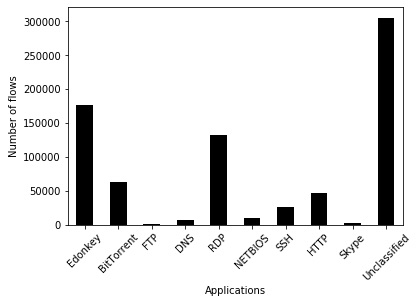
\includegraphics[width=3.6in]{fig1.jpg}
\caption{BroadBand Communication Research Group PCAP Data Flow}
\label{fig1}
}
\end{figure}

For the preprocessing of the supplied data, 8 kinds of application were selected based on the number of flows.
The 8 applications selected the application that has traffic of the actual network and the number of flow is more than 2000.
The 8 most common Label names are the Remote Desktop Protocol (RDP), Skype, SSH, Bittorrent, HTTP-Facebook, HTTP-Google, HTTP-Wikipedia and HTTP-Yahoo.
The application layer payload of the selected flow internal packet is filtered and extracted, and 8 application layer payload data files are generated using the extracted payload data.

\subsection{Learning Data Generation}\label
The process of converting the application layer payload data file created in the above section into input data suitable for deep learning learning will be described.
The application payload data file is divided into per packet unit and per flow unit, and each learning data is generated.
Flow is the same as the 5-tuple of the packet's header information, and packets generated within 3600 seconds of the previous packet are bundled into the same flow.
  
Each packet is extracted from each application layer payload data, and the elements of the payload data of the packet are grouped by 4 bits into one unit of learning data.
Therefore, one pixel of the learning data represents the number of 0 to 15.
One packet data collects pixelized data and image data as shown in Fig.\ref{fig2}.
One image data is converted into one packet learning data.

\begin{figure}[!t]
\centering
\setlength{\abovecaptionskip}{0pt}
\setlength{\belowcaptionskip}{0pt}
{
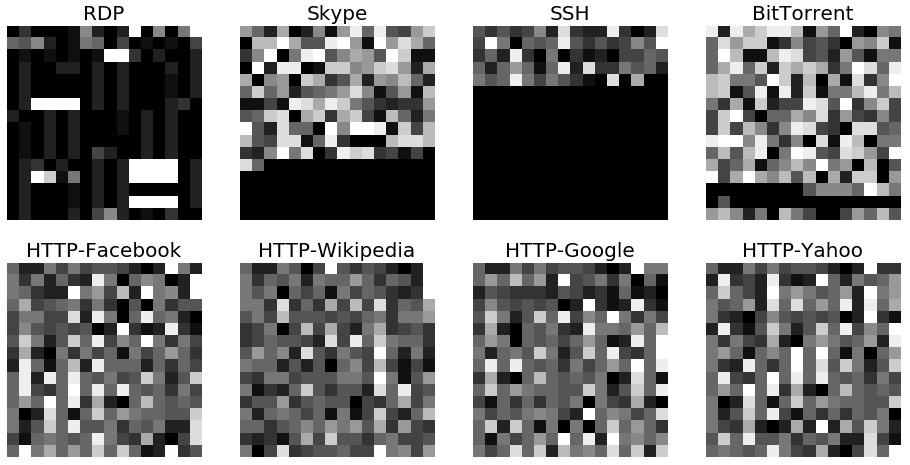
\includegraphics[width=3.6in]{fig2.jpg}
\caption{BroadBand Communication Research Group PCAP Data Flow}
\label{fig2}
}
\end{figure}

The learning data is generated by the packet unit and the flow unit for each application.
The learning data for each application per packet generates learning data by arbitrarily extracting packets of 8 applications (RDP, SSH, Skype, BitTorrent, Facebook, Wikipedia, Google, Yahoo) from the application layer payload data file.
In each application, 10000 random packets were extracted to extract a total of 80,000 learning data. One packet of each randomly extracted application is resized according to the size of the payload.
Therefore, the payload size of each application packet is extracted as 36 (6 * 6), 64 (8 * 8), 256 (16 * 16), and 1024 (32 * 32).
Figure 2 shows 16 * 16 of the payload data of an arbitrary packet for each extracted application.
If the extracted payload size is smaller than the set size, the size is adjusted by zero padding to match the set size.

The learning data of the flow unit is arbitrarily selected for each application in the application layer payload data file.
The selected flow fetches the packets from the first N packets as the number of packets (N) per predetermined flow.
They are  packets that has undergone a preprocessing process as in the learning data of each packet unit.
The learning data of the flow unit extracts 2000 flows for each application from the application layer payload data file and has a total of 16000 flows.
The number of N is set to 30, 60, and 100, and packets of each flow are fetched by the corresponding number to generate learning data.

Then, it is expressed as a one-hot vector with 8 lengths so that each of 8 applications can have label data.
A one-hot vector label is a vector with a value of only one element.
A one-value index can be defined as a label representing an application.
Therefore, two sets of learning data are used as the learning data packet or flow data and label data indicating the application data.